\chapter{TPTP Benchmarking}\label{chap:tptp-benchmarking}

The final part of this thesis work focuses on benchmarking the implementation of the fluted decision procedure, comparing its performance against Vampire (V4.9).

The TPTP (Thousands of Problems for Theorem Provers) library~\cite{Sut17} serves as the standard benchmark suite in automated theorem proving, containing a comprehensive collection of problems from various domains of mathematics and logic.
Beyond performance evaluation, the TPTP benchmark suite proved invaluable during the development process itself. By testing the implementation against known problems with established expected outcomes, we could verify the correctness of our fluted logic decision procedure at each development stage.

PTP contains many diverse problem formats, from first-order logic to typed higher-order logic. For our purposes only the first-order logic (FOF) and clause normal form (CNF) formats are relevant.
Problems are formulated in PROLOG-like syntax~\cite{Sut22}, making them both human-readable and machine-parsable.

FOF problems are expressed as a list of formulae, using a readable syntax where each of the formulae are enclosed within \code{fof(name, role, formula)} statements, with \code{name} being a unique identifier, \code{role} indicating the formula's purpose (such as \code{axiom}, \code{conjecture}, or \code{negated\_conjecture}), and \code{formula} containing the actual logical expression. %chktex 36
Variables are represented with capitalized word (such as \code{X}, \code{Y1}, \code{VarName}), while functions and predicate symbols use lowercase (like \code{a}, \code{pred}, \code{function\_name}).
Logical connectives include \code{\&} (\(\land\)), \code{|} (\(\lor\)), \code{=>} (\(\implies\)), \code{<=>} (\(\iff\)), and \textasciitilde{} (\(\neg\)).
Quantifiers are denoted by \code{!} for \(\forall\) and \code{?} for \(\exists\), with the quantified variables list following the quantifier within the square brackets (e.g.\ \code{[X1,X2]}). %chktex 36
Parentheses are used to ensure the correct order of operations and scope.
For example, the formula \(\forall x (P(x) \implies Q(f(x)))\) would be represented in TPTP FOF format as:
\begin{verbatim}
  fof(f1, axiom, ![X] (P(X) => Q(f(X)))).
\end{verbatim}
CNF problems follow a similar structure with the only difference being that instead of having formulae, they contain clauses expressed as disjunctions of literals. %chktex 36
For instance, the clausification of the previous formula would be represented as:
\begin{verbatim}
  cnf(c1, axiom, (~P(X) | Q(f(X)))).
\end{verbatim}
Problems are grouped into directories based on their domain of interest, such as \code{ALG} for general algebra, \code{KRS} for knowledge representation or \code{SYN} for syntax.

Obviously, not all problems in the library contain exclusively fluted formulae or clauses. Therefore, a classification step is necessary to filter out the relevant problems for our benchmarking purposes.

\section{Classifier}\label{sec:classifier}

For input problem classification, two possible approaches could have been considered.
The first involves parsing the TPTP files directly to identify fluted formulae and clauses, potentially using a high-level programming language with robust text processing libraries.
The second one, instead, was to leverage Vampire's existing parser and infrastructure to work with already tree-structured objects for formulae and list-structured objects for clauses.
The latter approach was ultimately chosen for its ease of integration with the existing codebase and potential reuse.

The main idea behind this classification process is, after correctly identifying if we are dealing with a FOF or CNF problem, to traverse each unit assuring all syntactic rules described in Sections~\ref{sec:fluted-formulae} and~\ref{sec:fluted-clauses} are respected.
For this purpose, two specific classes, \code{FormulaClassifier} and \code{ClauseClassifier}, were implemented. An additional general \code{Classifier} class was also added to handle dispatching.

\begin{figure}[H]
  \centering
  \includegraphics[width=0.8\textwidth]{6-tptp-benchmarking/Classifier.pdf}
  \caption{Class diagram of the \code{Classifier} class.}\label{fig:classifier-uml}
\end{figure}
\subsection{Formulae Classification}\label{subsec:formulae-classification}
As for formulae classification, we followed the approach mentioned at the end of Section~\ref{sec:fluted-formulae}, following the top-down depicted there.
Basically, the algorithm is a pre-order traversal of the formula tree, where in quantifier nodes variables are accumulated into a sequence, and in leaf nodes the argument list of the literal is checked against the accumulated sequence of variables to ensure it is a suffix of it.

\begin{algorithm}[H]
    \caption{\code{FormulaClassifier}'s classification methods}\label{alg:formula-classifier}
    \begin{algorithmic}[1]
        \Statex{} \bold{signature} \(\textsc{isInFlutedFragment:} \quad UnitList* \to Boolean\)
        \Function{\(\textsc{isInFlutedFragment}\)}{$ul$} % chktex 46
            \While{\(ul \neq \emptyset\)}
              \State{} \(vars \gets \emptyset\)
              \State{} \(u \gets ul.next()\)
              \If{\(\neg isFluted(u.getFormula(),vars)\)}
                \State{} \Return{} \(False\)
              \EndIf{}
            \EndWhile{}
            \State{} \Return{} \(True\)
        \EndFunction{}
    \end{algorithmic}

    \begin{algorithmic}[1]
        \Statex{} \bold{signature} \(\textsc{isFluted:} \quad Formula* \times VStack\to Boolean\)
        \Function{\(\textsc{isFluted}\)}{$formula,vars$} % chktex 46
            \Switch{\(formula.connective\)}
                \Case{\(\implies, \iff\)}
                    \State{} \(left \gets formula.left()\)
                    \State{} \(right \gets formula.right()\)
                    \State{} \Return{} \(isFluted(left,vars) \land isFluted(right,vars)\)
                \EndCase{}
                \Case{\(\neg\)}
                    \State{} \Return{} \(isFluted(formula.subformula(),vars)\)
                \EndCase{}
                \Case{\(\land, \lor\)}
                    \State{} \(subformulae \gets formula.subformulae()\)
                    \For{\(f \in subformulae\)}
                        \If{\(\neg isFluted(f,vars)\)}
                            \State{} \Return{} \(False\)
                        \EndIf{}
                    \EndFor{}
                    \State{} \Return{} \(True\)
                \EndCase{}
                \Case{\(\forall, \exists\)}
                    \For{\(v \in formula.quantifiedVariables()\)}
                        \State{} \(vars.push(v)\)
                    \EndFor{}
                    \State{} \Return{} \(isFluted(formula.subformula(),vars)\)
                \EndCase{}
                \Case{literal}
                    \State{} \Return{} \(isFluted(formula.literal(),vars)\)
                \EndCase{}
            \EndSwitch{}
        \EndFunction{}
    \end{algorithmic}
\end{algorithm}
\begin{algorithm}
  \caption{\code{FormulaClassifier}'s literals check}\label{alg:formula-classifier-literals}
  \begin{algorithmic}[1]
      \Statex{} \bold{signature} \(\textsc{isFluted:} \quad Literal* \times VStack\to Boolean\)
      \Function{\(\textsc{isFluted}\)}{$literal,vars$} % chktex 46
          \If{\(isEquality(literal)\)}
            \State{} \Return{} \(False\)
          \EndIf{}
          \State{} \(args \gets reverse(literal.arguments())\)
          \While{\(args \neq \emptyset \land vars \neq \emptyset\)}
              \State{} \(\arg \gets args.pop()\)
              \State{} \(v \gets vars.pop()\)
              \If{\(\arg \neq v\)}
                  \State{} \Return{} \(False\)
              \EndIf{}
          \EndWhile{}
          \State{} \Return{} \(args = \emptyset\)
      \EndFunction{}
  \end{algorithmic}
\end{algorithm}

To try to increase the number of problems found and consequently the size of the benchmark, we attempted to relax the fluted fragment constraints by introducing the concept of \emph{flutable formulae}.
As mentioned in Section~\ref{sec:fluted-formulae}, a formula is considered fluted even if it is not strictly fluted, but a variable renaming can transform it into a fluted formula.
For example the formula
\[
  \forall x_1,x_2 (P(x_1,x_2) \land \forall x_2,x_1 (Q(x_2,x_1)))
\]
may not appear fluted at first glance, but renaming the variables in the right-hand side subformula reversing them produces
\[
  \forall x_1,x_2 (P(x_1,x_2) \land \forall x_1,x_2 (Q(x_1,x_2)))
\]
which is fluted.
This is not the case, however, for formulae where the predicate variable lists do not match with the quantifiers quantifying those variables.
For example, for the formula
\[
  \forall x_1,x_2 P(x_2,x_1) 
\]
there is no variable renaming that can make it fluted, since the predicate arguments are in reversed order with respect to the quantifiers.
What would be needed is to permute the variables of the predicate so that they agree with the quantifiers, and this is exactly what defines a flutable formula.
\begin{definition}\label{def:flutable-formulae}
  A formula \(\phi\) is \emph{flutable} if there exists a permutation of the variables for each atomic formula in \(\phi\) that makes it fluted.
\end{definition}
For the previous example, the formula is flutable since applying the permutation \(\pi_P\) that swaps \(x_1\) and \(x_2\) will produce:
\[
  \forall x_1,x_2 P(x_1,x_2) 
\]
that is clearly fluted.
Despite these permutations do not always produce equivalent formulae, they preserve satisfiability.

\begin{lemma}
  Let \(\phi\) be a flutable formula, and \(\phi'\) the fluted formula obtained by applying a family of permutations on variables \(\pi\).
  Then \(\phi\) and \(\phi'\) are equisatisfiable.
\end{lemma}

\begin{proof}
  Suppose \(\phi\) is satisfiable.
  Being \(\phi\) satisfiable, there exists a model \(M = (D,I)\) such that \(M \models \phi\).
  From this, it is always possible to construct a model \(M' = (D,I')\) such that:
  
  for every predicate \(P \in \mathcal{P}\):
  \[I'(P) = \{(a_{\pi_P(1)}, a_{\pi_P(2)}, ..., a_{\pi_P(n_P)}) | (a_1, a_2, ..., a_{n_P}) \in I(P)\}\]

  This model \(M'\) is such that \(M' \models \phi'\).
  Suppose now that \(\phi\) is unsatisfiable and, for sake of contradiction, that \(\phi'\) is satisfiable.
  Analogously as described before, we can construct a model \(M\) such that \(M \models \phi\), from the model \(M'\) such that \(M' \models \phi'\), leading to a contradiction.
  \qed{}
\end{proof}

As stated in the Definition~\ref{def:flutable-formulae}, the permutation has to be applied homogeneously across all atomic formulae in \(\phi\).
Therefore, formulae like the one expressing the symmetric property:
\[
  \forall x_1,x_2 P(x_1,x_2) \iff (P(x_2,x_1))
\]
are neither fluted nor flutable, since there is no single permutation that can make both \(P\) and \(P\) fluted simultaneously.
Trivially, each fluted formula is also flutable, since the identity permutation can be applied.

To spot possible flutable formulae among the TPTP library, we implemented an additional method \code{isFlutable} in substitution of the \code{isFluted} overload that accepts literals.
This method builds the permutations needed to make the literals fluted, if possible, and checks if it is consistent with the permutations already found for previous occurred literals with the same signature in the formulae.
For doing so, a map data structure is used to store the variable correspondences, with.

\begin{algorithm}[H]
  \caption{\code{FormulaClassifier}'s literals check}\label{alg:formula-classifier-literals-flutable}
  \begin{algorithmic}[1]
      \Statex{} \bold{signature} \(\textsc{isFlutable:} \quad Literal* \times VStack\to Boolean\)
      \Function{\(\textsc{isFlutable}\)}{$literal,vars$} % chktex 46
          \If{\(isEquality(literal)\)}
            \State{} \Return{} \(False\)
          \EndIf{}
          \State{} \(args \gets reverse(literal.arguments())\)
          \State{} \((i,arity) \gets (|args|,|args|)\)
          \State{} \(perm \gets Array(arity)\)
          \While{\(i > 0 \land vars \neq \emptyset\)}
              \State{} \(i \gets i - 1\)
              \State{} \(\arg \gets args[i]\)
              \State{} \(v \gets vars.pop()\)
              \If{\(v \not\in literal.arguments() \lor v \in perm\)}
                  \State{} \Return{} \(False\)
              \EndIf{}
              \State{} \(idx \gets indexOf(v, literal.arguments())\)
              \State{} \(perm[i] \gets idx\)
          \EndWhile{}
          \If{\(i > 0\)}
            \State{} \Return{} \(False\)
          \EndIf{}
          \State{} \(prevPerm \gets \_permutationMap[literal.functor()]\)
          \If{\(isSome(prevPerm)\)}
            \If{\(prevPerm \neq perm\)}
              \State{} \Return{} \(False\)
            \EndIf{}
          \Else{}
            \State{} \(\_permutationMap[literal.functor()] \gets perm\)
          \EndIf{}
          \State{} \Return{} \(True\)
      \EndFunction{}
  \end{algorithmic}
\end{algorithm}

To use flutable problems, another preprocessing step would have been necessary, to apply all the found permutations.
This one though was not implemented, since no additional non-fluted flutable problem was found in TPTP version 9.0.0.

\subsection{Clauses Classification}\label{subsec:clauses-classification}

Clause classification was a considerably more difficult task. This is because, to be a fluted, a clause have three possible condition to satisfy, as described in Section~\ref{sec:fluted-clauses}.
Moreover, for (FL2)-clauses, we had to account for constructing a fluted sequence that remained coherent throughout the clause.
To facilitate the implementation, we introduced two new classes: \code{EVar}, already mentioned in Section~\ref{sec:separation-impl}, to represent an \emph{extended variable}, and \code{FlutedSequence}, to represent a fluted sequence.

\code{EVar} can be seen as a wrapper of type \code{Variable | Constant | Nothing}, representing either a variable, usually the extremes of the variable section of a fluted sequence, a constant, and so the fluted sequences over \(X_0\), or nothing for the time in the algorithm when a variable was not set yet.
Furthermore, it provides some utility methods to check its type and check the \emph{distance} with other \code{EVar} instances, where distance can be seen as the absolute value of the difference between their positions in \(X_m\), with constants being before all variables.

\code{FlutedSequence} is a more complex structure that contains an \code{EVar} representing the last variable in the sequence, and a list of \code{Term} for the functional parts.
Other than exposing all \code{EVar} methods, it also provides methods to manipulate the sequence, such as adding or removing functional parts, and checking, given another list of \code{Term}, the prefix and suffix relations.
This will come in handy when checking if two functional (FL2)-literals share a compatible fluted sequence and if all subterms have argument sequences suffixes of the running sequence.

The first method \code{isFluted} accepts a clause and checks which condition the clause can possibly satisfy.

\begin{algorithm}
  \algnotext{EndIf}
  \algnotext{EndFunction}
  \algnotext{EndWhile}
  \algnotext{EndFor}
  \algnotext{EndCase}
  \algnotext{EndSwitch}
  \caption{Fluted Clause Detection}
  \begin{algorithmic}[1]
      \Statex{} \bold{signature} \(\textsc{isFlutable:} \quad Clause* \to Boolean\)
      \Function{\(\textsc{isFlutable}\)}{$cl$} % chktex 46
        \State{} \(lits \gets cl.literals()\)
        \State{} \(l \gets lits.next()\)
        \If{\(isEquality(l)\)}
          \State{} \Return{} \(False\)
        \EndIf{}
        \If{\(\neg allArgumentsAreVariable(l)\)}
          \State{} \Return{} \(isFL2(cl)\)
        \EndIf{}
        \State{} \(lastVar \gets EVar(l.lastArgument())\)
        \While{\(lits \neq \emptyset\)}
          \If{\(isEquality(l)\)}
            \State{} \Return{} \(False\)
          \EndIf{}
          \If{\(\neg allArgumentsAreVariable(l)\)}
            \State{} \Return{} \(isFL2(cl)\)
          \EndIf{}
          \State{} \(var \gets EVar(l.lastArgument())\)
          \If{\(var \neq lastVar \land lastVar.distance(var) = 1\)}
            \State{} \Return{} \(isFL3(cl)\)
          \EndIf{}
        \EndWhile{}
        \State{} \Return{} \(isFL1(cl)\)
      \EndFunction{}
  \end{algorithmic}
\end{algorithm}

Regarding (FL1)-clauses, the detection is simpler since it only requires checking if all arguments are variables in correct order.

\begin{algorithm}[H]
  \caption{Checking (FL1)-clauses}
  \begin{algorithmic}[1]
      \Statex{} \bold{signature} \(\textsc{isFL1:} \quad Clause* \to Boolean\)
      \Function{\(\textsc{isFL1}\)}{$cl$} % chktex 46
        \State{} \(seq \gets FlutedSequence()\)
        \State{} \(lits \gets cl.literals()\)
        \While{\(lits \neq \emptyset\)}
          \State{} \(l \gets lits.next()\)
          \If{\(isEquality(l) \lor \neg allArgumentsAreVariable(l)\)}
            \State{} \Return{} \(False\)
          \EndIf{}
          \If{\(varsSeqHasHoles(l)\)}
            \State{} \Return{} \(False\)
          \EndIf{}
          \If{\(seq.isVarSet()\)}
            \If{\(l.lastArgument() \neq seq.var()\)}
              \State{} \Return{} \(False\)
            \EndIf{}
          \Else{}
            \State{} \(seq.setVar(EVar(l.lastArgument()))\)
          \EndIf{}
        \EndWhile{}
        \State{} \Return{} \(True\)
      \EndFunction{}
  \end{algorithmic}
\end{algorithm}

The (FL3)-clauses detection is also quite straightforward, as it only requires the additional check that the distance between the rightmost variables of two literals is at most 1.
The only caution to have is to avoid relaying on transitivity for these checks, because it could lead to incorrect results.
As an example, consider the clause:
\[
P(x_1,x_2) \lor Q(x_2,x_3) \lor R(x_3,x_4)
\]

This clause is not fluted, because the distance between the rightmost variables of \(P\) and \(R\) is 2, even though the distances between \(P\) and \(Q\), and between \(Q\) and \(R\) are both 1.

To achieve this tracking using two \code{EVar} instances, keeping the invariant that the first one is the smaller of the two and that once both are set, they are not changed.
The compatibility verification is performed by the method \code{updateRightMostVars} (Algorithm~\ref{alg:updateRightMostVars}), which takes the two \code{EVar} instances while checking if the new rightmost variable found is compatible with the variable found since the last update.

Laid down this method, verifying if a clause is (FL3) is just a matter of iterating through the literals, checking that all arguments are variables in correct order, and updating the rightmost variables accordingly.
\begin{algorithm}[H]
  \algnotext{EndIf}
  \algnotext{EndFunction}
  \algnotext{EndWhile}
  \algnotext{EndFor}
  \algnotext{EndCase}
  \algnotext{EndSwitch}
  \caption{Updating rightmost variables}\label{alg:updateRightMostVars}
  \begin{algorithmic}[1]
      \Statex{} \bold{signature} \(\textsc{updateRightMostVars:} \quad EVar \times EVar \times Variable \to Boolean\)
      \Function{\(\textsc{updateRightMostVars}\)}{$var1, var2, newVar$} % chktex 46
        \If{\(var1.isSet() \land var2.isSet()\)}
          \If{\(var1.var() \neq newVar \land var2.var() \neq newVar\)}
            \State{} \Return{} \(False\)
          \EndIf{}
        \ElsIf{\(var1.isSet()\)}
          \Switch{\(var1.distance(lastVar)\)}
            \Case{\(1\)}
              \If{\(var1.var() < newVar\)}
                \State{} \(var2.set(newVar)\)
              \Else{}
                \State{} \(var2.set(var1.var())\)
                \State{} \(var1.set(newVar)\)
              \EndIf{}
            \EndCase{}
            \Case{\(0\)}
              \State{} \Return{} \(True\)
            \EndCase{}
            \Default{}
              \State{} \Return{} \(False\)
            \EndDefault{}
          \EndSwitch{}
        \Else{}
          \State{} \(var1.set(newVar)\)
          \EndIf{}
        \State{} \Return{} \(True\)
      \EndFunction{}
  \end{algorithmic}
\end{algorithm}

\begin{algorithm}[H]
  \algnotext{EndIf}
  \algnotext{EndFunction}
  \algnotext{EndWhile}
  \algnotext{EndFor}
  \algnotext{EndCase}
  \algnotext{EndSwitch}
  \caption{Checking (FL3)-clauses}
  \begin{algorithmic}[1]
      \Statex{} \bold{signature} \(\textsc{isFL3:} \quad Clause* \to Boolean\)
      \Function{\(\textsc{isFL3}\)}{$cl$} % chktex 46
        \State{} \(lits \gets cl.literals()\)
        \State{} \((rm1,rm2) \gets (EVar(),EVar())\)
        \While{\(lits \neq \emptyset\)}
          \State{} \(l \gets lits.next()\)
          \If{\(isEquality(l) \lor \neg allArgumentsAreVariable(l)\)}
            \State{} \Return{} \(False\)
          \EndIf{}
          \State{} \(vars \gets l.arguments()\)
          \If{\(varsSeqHasHoles(l)\)}
            \State{} \Return{} \(False\)
          \EndIf{}
          \State{} \(newVar \gets l.lastArgument()\)
          \If{\(\neg updateRightMostVars(rm1,rm2,newVar)\)}
            \State{} \Return{} \(False\)
          \EndIf{}
        \EndWhile{}
        \State{} \Return{} \(True\)
      \EndFunction{}
  \end{algorithmic}
\end{algorithm}

Finally, the (FL2)-clauses detection is the most complex one. This process has been separated into two procedures: one internal loop through the subterm of a literal, building an internal fluted sequence, and an external loop through the literals of the clause, checking that all literals share a compatible fluted sequence.
This traversal of can be seen as a depth-first search with repetition in a graph. With each literal represented as a DAG, standard techniques to avoid loops such as node colouring are superfluous.
Moreover, the traversal can leverage the diverse nature of nodes, where predicate nodes are the only \dquote{entry points} to the graph, and term nodes are the only internal nodes.
For the sake of brevity, these two functions are shown at a higher level of abstraction, omitting some details.

\begin{algorithm}[H]
  \algnotext{EndIf}
  \algnotext{EndFunction}
  \algnotext{EndWhile}
  \algnotext{EndFor}
  \algnotext{EndCase}
  \algnotext{EndSwitch}
  \caption{(FL2)-literal internal loop}\label{alg:fl2-internal}
  \begin{algorithmic}[1]
      \Statex{} \bold{signature} \(\textsc{isFluted:} \quad Term* \times EVar \to FlutedSequence | False\)
      \Function{\(\textsc{isFluted}\)}{$term,v$} % chktex 46
        \State{} \(isFunctional \gets False\)
        \State{} \(args \gets term.subterms()\)
        \State{} \(\arg \gets args.next()\)
        \State{} \(currVar \gets EVar()\)
        \State{} \((localSeq,internalSeq) \gets (FlutedSequence(),FlutedSequence())\)
        \If{\(\arg.isFunctional()\)}
          \State{} \(isFunctional \gets True\)
          \State{} \(localSeq.add(\arg)\)
        \Else{}
          \State{} \(currVar \gets \arg.var()\)
        \EndIf{}
        \While{\(args \neq \emptyset\)}
          \State{} \(\arg \gets args.next()\)
          \If{\(\arg.isFunctional()\)}
            \State{} \(isFunctional \gets True\)
            \State{} \(innerSeq \gets isFluted(\arg, v)\)
            \Comment{} Recursively check subterms
            \If{\(\neg innerSeq.isValid()\)}
              \State{} \Return{} \(False\)
            \EndIf{}
            \If{\(\neg innerSeq.isSuffixOf(localSeq)\)}
              \State{} \Return{} \(False\)
            \EndIf{}
            \State{} \(localSeq.add(\arg)\)
          \Else{}
            \State{} \(currVar \gets currVar +1\)
            \If{\(isFunctional \lor currVar \neq \arg.var() \lor v > currVar\)}
              \State{} \Return{} \(False\)
            \EndIf{}
          \EndIf{}
        \EndWhile{}
        \If{\(\neg v.isSet() \land currVar.isSet()\)}
          \State{} \(v.set(currVar)\)
        \EndIf{}
        \State{} \(localSeq.setVar(v)\)
        \State{} \Return{} \(localSeq\)
      \EndFunction{}
  \end{algorithmic}
\end{algorithm}

Algorithm~\ref{alg:fl2-internal} recursively traverses each term building the local fluted sequence, keeping track of the rightmost variable in the fluted sequence and updating the list of functional term after each term is verified.
When a subterm completes successfully the construction of its local fluted sequence, it is returned to be checked against the current local fluted sequence of the parent term, to assure that is a suffix of it.
Otherwise, the function implements early exiting by returning \(False\) as soon as an invalid condition is detected.
Finally, if the rightmost variable is not set yet, it is updated with the one found in the current term.

\begin{algorithm}[H]
  \algnotext{EndIf}
  \algnotext{EndFunction}
  \algnotext{EndWhile}
  \algnotext{EndFor}
  \algnotext{EndCase}
  \algnotext{EndSwitch}
  \caption{(FL2)-literal external loop}\label{alg:fl2-external}
  \begin{algorithmic}[1]
      \Statex{} \bold{signature} \(\textsc{isFL2:} \quad Clause* \to Boolean\)
      \Function{\(\textsc{isFL2}\)}{$cl$} % chktex 46
        \State{} \(lit \gets cl.literals()\)
        \State{} \(localSeq \gets FlutedSequence()\)
        \While{\(lit \neq \emptyset\)}
          \State{} \(currLit \gets lit.next()\)
          \If{\(isEquality(currLit)\)}
            \State{} \Return{} \(False\)
          \EndIf{}
          \If{\(allArgumentsAreVariable(currLit)\)}
            \Comment{This case is in \(\nabla\)}
            \If{\(varsSeqHasHoles(currLit, localSeq)\)}
              \State{} \Return{} \(False\)
            \Else{}
              \State{} \(localSeq.setVar(currLit.lastArgument())\)
            \EndIf{}
          \Else{}
            \State{} \(innerSeq \gets isFluted(currLit, localSeq.var())\)
            \If{\(\neg innerSeq.isValid() \)}
              \State{} \Return{} \(False\)
            \EndIf{}
            \If{\(\neg localSeq.isVarSet()\)}
              \State{} \(localSeq.setVar(innerSeq.var())\)
            \ElsIf{\(localSeq.var() \neq innerSeq.var()\)}
              \State{} \Return{} \(False\)
            \EndIf{}
            \If{\(localSeq.hasTermLists()\)}
              \State{} \(localSeq.setTermList(innerSeq)\)
            \Else{}
              \If{\(\neg onePrefixOfOther(localSeq, innerSeq)\)}
                \State{} \Return{} \(False\)
              \Else{}
                \State{} \(newSeq \gets longest(localSeq.termList(), innerSeq.termList())\)
                \State{} \(localSeq.setTermList(newSeq)\)
              \EndIf{}
            \EndIf{}
          \EndIf{}
        \EndWhile{}
        \State{} \Return{} \(True\)
      \EndFunction{}
  \end{algorithmic}
\end{algorithm}

\section{Experimental Setup}\label{sec:tptp-experimental-setup}

After implementing the classifier described in Section~\ref{sec:classifier}, we applied it to the TPTP library version 9.0.0 to identify problems suitable for fluted logic benchmarking.
The TPTP library provides a useful prefiltering script \code{tptp2t} that allows filtering problems by various criteria, which can be used to initially exclude problems containing undesirable features.
In our case, we used it to filter out problems containing equality and purely propositional CNF problems, with the commands:
\begin{verbatim}
  tptp2T -q2 -pp Form FOF -Equality
  tptp2T -q2 -pp Form CNF -Equality -Propositional
\end{verbatim}

These commands outputted \(1969\) and \(2222\) problems, respectively, which we then classified, arriving at a total of only \(128\) FOF problems, of which \(26\) purely propositional, and just \(23\) CNF problems being fluted.
These problems, reported in Appendix~\ref{app:fluted-problems}, are distributed across the various domains as shown in Tables~\ref{tab:fof_distribution} and~\ref{tab:cnf_distribution}.
% filepath: /Volumes/Hard Disk Esterno/Thesis/_chapters/6-tptp-benchmarking.tex
\begin{table}[H]
  \centering
  \begin{minipage}[t]{0.48\textwidth}
    \centering
    \caption{FOF Problems Distribution}\label{tab:fof_distribution}
    \begin{tabular}{l r}
      \toprule
      Domain & Count \\
      \midrule
      KRS & 22 \\
      LCL & 10 (3 prop.) \\
      MSC & 2 \\
      SYN & 94 (23 prop.) \\
      \midrule
      \bold{Total} & \bold{128} \\
      \bottomrule
    \end{tabular}
  \end{minipage}
  \hfill
  \begin{minipage}[t]{0.48\textwidth}
    \centering
    \caption{CNF Problems Distribution}\label{tab:cnf_distribution}
    \begin{tabular}{l r}
      \toprule
      Domain & Count \\
      \midrule
      COM & 2 \\
      KRS & 1 \\
      PUZ & 1 \\
      SYN & 19 \\
      \midrule
      \bold{Total} & \bold{23} \\
      \bottomrule
    \end{tabular}
  \end{minipage}
\end{table}

Because of this lack of test cases, we consider generating our own fluted problems, which will be covered in Chapter~\ref{chap:generated-benchmarking}.

To ensure that no optimization or heuristic in Vampire was unfairly advantaging or disadvantaging neither our implementation nor the original Vampire system, we had to disable some options.
In particular, the disabled options are:
\begin{itemize}
  \item unused predicate definition removal, to prevent a possible interference with our naming procedure;
  \item forward subsumption and forward subsumption resolution, to assure that only resolution and factoring are used;
  \item avatar splitting, as previously mentioned, to avoid the use of propositional reasoning.
\end{itemize}

Alongside these settings, other options related to equality have been disabled being irrelevant for our problems.
Finally, exclusively for fluted resolution, we had to use \code{any} as literal selection option, to avoid possible conflicts with our selection method.

As for the saturation algorithm used, having very few test cases, we had the opportunity to experiment with both \emph{Otter} and \emph{LRS} strategies, to analyse potential performance differences.

The tests have been run on a machine with an Apple M1 Pro CPU with 8 cores and 8 GB of RAM, with a timeout of \(300\) seconds.
For each problem, we run the solver 5 times to average out any variability in execution time, taking the average of these runs as the final result.
In addition, for problems that lead to an error or crash, we used the symbolic value of \(330\) seconds to indicate that the problem was not solved, allowing us to include these cases in the performance charts.

\section{Results and Analysis}\label{sec:tptp-results-analysis}

The following graphs show the general trends of the experiments, confronting both Vampire and fluted resolution, using either \emph{Otter} or \emph{LRS} as saturation algorithm.
A complete table of the results is available in Appendix~\ref{app:benchmark-results}.

The first comparison is between Vampire and fluted resolution using the \emph{LRS} strategy for FOF problems, shown in Figure~\ref{fig:fof-lrs}.

As it is possible to see from the charts, both Vampire and fluted resolution alternate between immediate terminations with timeouts.
Regarding CNF problems, shown in Figure~\ref{fig:cnf-lrs}, the two are nearly identical in performance, with the only difference being in Vampire performing sufficiently better on problem SYN328--1.
Contrarily, for FOF problems, Vampire is outperformed by fluted resolution in most cases, with the only exception being problems KRS019+1 and SYN007+1, where the cause of the failure seems to be the preprocessing step.
That problem is actually full of biconditionals, which are ignored by the version of structural transformation we implemented. This lead to a blow-up in the number of clauses generated, running out of resources quickly.
\begin{figure}[H]
  \centering
  \includegraphics[width=\textwidth]{6-tptp-benchmarking/fof/0-lrs_comparison.png}
  \caption{FOF Problems solved using LRS strategy.}\label{fig:fof-lrs}
\end{figure}

\begin{figure}[H]
  \centering
  \includegraphics[width=\textwidth]{6-tptp-benchmarking/cnf/0-lrs_comparison.png}
  \caption{CNF Problems solved using LRS strategy.}\label{fig:cnf-lrs}
\end{figure}



Continuing with the analysis of the results, we have the comparison between Vampire and fluted resolution using the \emph{Otter} strategy, shown in Figures~\ref{fig:fof-otter} and~\ref{fig:cnf-otter}.

\begin{figure}[H]
  \centering
  \includegraphics[width=\textwidth]{6-tptp-benchmarking/fof/1-otter_comparison.png}
  \caption{FOF Problems solved using Otter strategy.}\label{fig:fof-otter}
\end{figure}

\begin{figure}[H]
  \centering
  \includegraphics[width=\textwidth]{6-tptp-benchmarking/cnf/1-otter_comparison.png}
  \caption{CNF Problems solved using Otter strategy.}\label{fig:cnf-otter}
\end{figure}

Comparing the general performance of the two strategies, it is immediately noticeable that the change in strategy did not have a significant impact on the overall results. Both strategies exhibit similar patterns in terms of problem-solving capabilities, with only minor variations in specific cases.
Some specific problems though, have substantially different results.

For CNF problems, in the only test case where Vampire and fluted resolution exhibit a notable gap, their performances difference is accentuated. This is probably due to the fact that the \emph{LRS} strategy deleted as unreachable some clauses used by Vampire with \emph{Otter} to solve the problem earlier.
On the front of FOF instead, we can see this behaviour exhibited by fluted resolution, in problem KRS132+1, improving its performance from being over 3 minutes to under 1 minute. Another slight improvement can be observed in Vampire's performance on problem SYN392+1, avoiding the timeout previously encountered for just 20 seconds.

Another important thing to mention is that, moving to the \emph{Otter} strategy, problem SYN007+1, one of the two FOF where Vampire outperformed fluted resolution, is now unsolved by both systems. This evidence, combined with the countless timeout become errors or crush, highlights the impact and the importance of the \emph{LRS} strategy.

This difference is made even more evident by comparing the performances of both Vampire and fluted resolution using the two strategies, as shown in next charts.

\begin{figure}[H]
  \centering
  \includegraphics[width=\textwidth]{6-tptp-benchmarking/fof/2-fluted_comparison.png}
  \caption{FOF Problems solved using fluted resolution with different strategies.}\label{fig:fof-fluted}
\end{figure}

\begin{figure}[H]
  \centering
  \includegraphics[width=\textwidth]{6-tptp-benchmarking/cnf/2-fluted_comparison.png}
  \caption{CNF Problems solved using fluted resolution with different strategies.}\label{fig:cnf-fluted}
\end{figure}
\begin{figure}[H]
  \centering
  \includegraphics[width=\textwidth]{6-tptp-benchmarking/fof/3-vampire_comparison.png}
  \caption{FOF Problems solved using Vampire's resolution with different strategies.}\label{fig:fof-vampire}
\end{figure}

\begin{figure}[H]
  \centering
  \includegraphics[width=\textwidth]{6-tptp-benchmarking/cnf/3-vampire_comparison.png}
  \caption{CNF Problems solved using Vampire's resolution with different strategies.}\label{fig:cnf-vampire}
\end{figure}

The experimental results demonstrate that the fluted resolution implementation successfully keeps pace with Vampire, the established standard in automated theorem proving.
A quantitative analysis of the benchmark results reveals that fluted resolution outperforms Vampire in more test cases than it underperforms, suggesting competitive performance across the evaluated problem sets.
However, the results exhibit a highly polarized distribution, with solvers typically either solving problems almost instantaneously or timing out completely, making it difficult to discern clear performance trends or identify specific problem characteristics that favour one approach over the other.

While these initial results are promising, the limited number of test cases—comprising only a subset of TPTP problems—restricts the generalizability of our findings.
The binary nature of the outcomes (quick success versus timeout) provides insufficient granularity to conduct meaningful statistical analysis or to establish robust performance patterns.
To address these limitations and obtain more comprehensive insights into the comparative performance of fluted resolution, Chapter~\ref{chap:generated-benchmarking} presents the development of a systematic problem generator that enables large-scale evaluation across diverse problem structures and complexities.
